\documentclass[14pt,a4paper]{scrartcl}
\renewcommand{\sfdefault}{cmr}

\usepackage[utf8]{inputenc}
\usepackage[english,russian]{babel}

\usepackage{indentfirst}
\usepackage{graphicx}
\usepackage{misccorr}
\usepackage{amsmath}
\usepackage{amssymb}
\usepackage{amsfonts}
\usepackage{icomma}
\usepackage{alltt}
\usepackage{enumitem}
\usepackage{soul}
\usepackage{soulutf8}
\usepackage{titlesec}

\titleformat
	{\section}
	[hang]
	{\normalfont\bfseries}
	{ \thesection.}{ }{}
\titlespacing
	{\section}
	{\parindent}
	{4ex}
	{0pt}
	
\titleformat
	{\subsection}
	[hang]
	{\normalfont\bfseries}
	{ \thesection.}{ }{}
\titlespacing
	{\subsection}
	{\parindent}
	{4ex}
	{0pt}
	
\titleformat
	{\subsubsection}
	[hang]
	{\normalfont\bfseries}
	{ \thesection.}{ }{}
\titlespacing
	{\subsubsection}
	{\parindent}
	{4ex}
	{0pt}

\begin{document}
	\begin{flushright}
	\textbf{Билеты по физической химии\\
		Залецкая Евгения \\
		Факультет химии, 1 курс}
\end{flushright}  	
\section*{Вопрос №1}
	
	\subsection*{Основные задачи химической термодинамики.} 
	Термодинамика изучает количественные соотношения между
	теплотой, работой и различными формами энергии, в том числе
	и химической. \\
	Химическая термодинамика изучает превращение энергии
	химических реакций в теплоту и работу. \\
	Основные задачи:
	\begin{itemize}
		\item Определение условий реализации химических процессов. Вычисление тепловых эффектор химических реакций.
		\item Поиск пределов устойчивости исследуемых веществ при заданных условиях.
		\item Избрание оптимального режима проведения процесса.	
	\end{itemize}
	
	\subsection*{Термодинамические параметры.} 
	\begin{itemize}
		\item Энтальпия
		\item Энтропия
		\item Энергия Гиббса
		\item Теплоемкость
	\end{itemize}
	
	\subsection*{Классификация систем.} 
	Под термодинамической системой (ТС) понимается некоторая часть пространства со всеми включенными в нее компонентами. Всякая ТС должна быть ограничена реальной или вооброжаемой границей - поверхностью раздела. Через поверхность может осуществляться обмен веществом или энергией.
	\begin{itemize}
		\item Открытая система -- ТС, в которой разрешены все типы обмена.
		\item Замкнутая система -- ТС, в которой разрешен только обмен энергией.
		\item Адиабатическая система -- ТС, в которой разрешен только обмен веществом.
		\item Изолированная система -- ТС, в которой запрещены любые обмены.
	\end{itemize}
	
	\subsection*{Экстенсивные и интенсивные термодинамические параметры.} 
	Для полного описания системы мы выбираем минимальный набор параметров - независимых переменных (который зависит от условий эксперимента). Назовем их параметрами состояния.
	\begin{itemize}
		\item Экстенсивные параметры состояния (ЭПС) - параметры, определяемые количеством вещества в системе: $ V, m, l, S, q  $. ЭПС аддитивны.
		\item Интенсивные параметры состояния (ИПС) - параметры, которые не зависят от количества вещества и могут быть измерены лишь опосредовано через ЭПС. Примеры: $p, T $
	\end{itemize}
	Любые виды работы ($A$) могут быть охарактеризованы так: (где Y - ИПС, а Х - ЭПС):
	$$ dA = Y dX  $$ 
	Например:
	$$ dA = P dV  $$
	\subsection*{Внутренняя энергия.} 
	Каждое вещество характеризуется потенциальным запасом энергии. Она включает в себя все виды энергии движения и взаимодействия частиц. Эта величина - внутренняя энергия ($U$). Она зависит только от термодинамических параметров ТС и не зависит от путей достижения конкретного состояния ТС, а значит $U$ - функция состояния. \\
	Мы никогда не работаем с абсолютными значениями $U$, а лишь с ее изменениями $\Delta{U}$.
		


	\section*{Вопрос №2}
	\subsection*{Первый закон термодинамики.} 
	Приведу две формулировки:
	\begin{itemize}
		\item В ходе любого процесса изменение внутренней энергии ТС равно разности между количеством сообщенной ей теплоты ($Q$) и совершенной ею работой ($A$):
		$$ (U_2 - U_1) = \Delta{U} = Q - A $$
		\item Сообщенная ТС теплота ($Q$) расходуется на изменение внутренней энергии ТС и совершение работы ($A$):
		$$ Q = \Delta{U} + A $$
	\end{itemize}
	\subsection*{Функция энтальпии.} 	
	Энтальпия ($H$) - функция состояния:
	$$ H = U + pV $$
	Использование энтальпии целесообразно, если ТС совершает  работу по сжатию/расширению, т.к. при $p = const$:
	$$ A = p \Delta{V} = \Delta{(pV)}  $$ 
	Добавим изменение внутренней энергии:
	$$Q = \Delta{U} + A = \Delta{U} + \Delta{(pV)} = \Delta{U + pV} = \Delta{H} $$
	\underline{Энтальпия - мера теплоты процесса, происходящего при постоянном давлении.} 
	
	\subsection*{Тепловой эффект химической реакции при постоянном давлении/объеме/температуре.} 
	\begin{itemize}
		\item При $p = const$: $Q = \Delta{H}$
		\item При $V = const$: $Q = \Delta{U}$, т.к. ТС не совершает работы.
		\item При $T = const$: $Q = A$, т.к. $U$ зависит от $T$ и при $T=const$ : $\Delta{U} = 0$.
	\end{itemize}
	
	\subsection*{Термохимические уравнения.}
	Термохимическое уравнение - уравнение с указанием теплового эффекта. (!) Тепловой эффект отнесен к 1 молю вещества.\\
	В термохимических уравнениях необходимо указывать агрегатные состояния исходных веществ и продуктов реакции. \\
	Существуют экзо- и энотермические реакции:
	\begin{itemize}
		\item Экзотермические реакции происходят с выделением тепла ($\Delta{U}, \Delta{H} < 0$)
		\item Эндотермические реакции происходят с поглощением тепла ($\Delta{U}, \Delta{H} > 0$)
	\end{itemize}
	\subsection*{Теплоты образования и сгорания. Стандартные теплоты и стандартные состояния.}
	\begin{itemize}
		\item Теплота образования -- тепловой эффект реакции образования 1 моля вещества из простых веществ.
		\item Теплота сгорания -- тепловой эффект реакции сгорания одного моля вещества в кислороде до образования оксидов в высшей степени окисления. Теплота сгорания негорючих веществ принимается равной нулю.
		\item Стандартная теплота образования -- тепловой эффект реакции образования одного моля вещества из простых веществ, его составляющих, находящихся в \underline{устойчивых стандартных состояниях.}
		\item Cтандартные состояния -- условно принятые состояния индивидуальных веществ и компонентов растворов при оценке термодинамических величин.  
		Например, для стандартных условий стандартное состояние углерода -- графит, т.к. для стандартных $p$ и $T$ это равновесная модификация углерода.
		Стандартные условия:
		\begin{itemize}
			\item $p = 10^5$ Па
			\item $T = 273,15 K$
		\end{itemize}
	\end{itemize}
	\subsection*{Энергия разрыва химической связи.}
	Энергия химической связи -- мольный прирост энергии вещества при разрушении одной связи определенного типа в каждой молекуле.			


\section*{Вопрос №3}	

		\subsection*{Расчет тепловых эффектов реакций по теплотам образования, сгорания и разрыва химических связей.}
		\begin{itemize}
			\item По теплотам образования: 
			$$\Delta{H_{p}^{o}} = \sum \Delta{H_{f}^o} \text{(продукты)} - \sum \Delta{H_{f}^o} \text{(реагенты)}  $$
			\item По теплотам сгорания: \\
			Аналогично первому методу, только необходимо брать энтальпию сгорания.
			\item По энергии химических связей:
			Зная состав и химическую формулу (со всеми связями между атомами вещества) можно оценить, какова его энергия формирования. Точные значения энергий конкретных связей -- справочная информация, но известно, что по силе взаимодействия:
			$$ -  <  =  <  \equiv $$
		\end{itemize}
		\subsection*{Закон Гесса и термохимия.} 
		Закон Гесса: \\
		Тепловой эффект химического процесса зависит только от природы и состояний исходных веществ и продуктов, но не от пути его осуществления, в том числе от выбора системы реакций и состояния промежуточных продуктов. \\
		Пример расчетов: \\
		$$C\text{(графит)} + \frac{1}{2}O_2\text{(г)} = CO\text{(г)}: \Delta{H_1}$$  
		$$C\text{(графит)} + \frac{1}{2}O_2\text{(г)} = CO_2\text{(г)}: \Delta{H_2} = -393,5 \text{кДж/моль}$$  			
		$$CO\text{(г)} + \frac{1}{2}O_2\text{(г)} = CO_2\text{(г)}: \Delta{H_3} = -110,5 \text{кДж/моль} $$  
		Отсюда:
		$$\Delta{H_1} = \Delta{H_2} - \Delta{H_3} $$
		\subsection*{Теплоемкость.} 		
		Истинная теплоемкость:
		$$C_T = \dfrac{dQ}{dT} $$
		Т.е. отношение теплоты ($dQ$), которая требуется, чтобы нагреть ТС на $dT$ к изменению температуры ($dT$). Тогда чтобы нагреть ТС от температуры $T_1$ до $T_2$:
		$$ Q = \int\limits_{T_1}^{T_2} C_T dT $$
		\subsection*{Теплоемкость идеального газа.} 
		Следует различать теплоемкость при постоянном давлении ($C_p$) и теплоемкость при постоянном объеме ($C_V$). Т.к. при $p=const$ теплота также расходуется на работу расширения. Поэтому:
		$$C_V = \dfrac{\frac{dU}{dT}}{n} $$
		$$C_p = \dfrac{\frac{dH}{dT}}{n} $$
		где $n$ - количество вещества. Для твердых и жидких веществ $C_p \approx C_V$. Для 1 моля идеального газа:
		$$C_p = \dfrac{dH}{dT} = \dfrac{d(U+pV)}{dT} = \dfrac{d(U+RT)}{dT} = \dfrac{dU}{dT} + R = C_V + R $$
		\subsection*{Теплоемкость одноатомного и многоатомных газов.} 
		Из МКТ известно, что:
		$$E = \dfrac{3}{2} kT \Rightarrow \Delta{U} = \dfrac{3}{2} RT $$
		Из теплоемкости идеального газа следует, что для одноатомного газа $C_V = \frac{3}{2} R $ и $C_p = \frac{5}{2}R$. На каждую поступательную степень свободы - $\frac{1}{2} R$. Столько же приходится и на вращательные. Тогда если в молекуле газа $N$ атомов $\Rightarrow 3N$ степеней свободы:
		$$ C_V = \dfrac{3N}{2} R $$
		$$ C_p = \dfrac{3N+2}{2} R $$
		Однако эти соотношения работают при больших температурах, при низких нужно учитывать вклад только вращательных степеней свободы, которых для линейных молекул 2, а для нелинейных -- 3.
		\subsection*{Зависимость теплоемкости и энтальпии вещества от температуры.} 
		\subsection*{Общие понятия о фазовых переходах} 		
		\subsection*{Зависимость тепловых эффектов химических реакций от температуры.} 		
		\subsection*{Уравнение Кирхгоффа.} 		


	\section*{Вопрос №4}
	
	\subsection*{Второй закон термодинамики} 
	Существуют некоторые процессы, не противоречащие первому закону термодинамики, которые самопроизвольно протекать не могут.\\ \\
	Процессы, которые не могут протекать самопроизвольно -- отрицательные. Отрицательный процесс не может являться единственным результатом действия. \\
	Постулаты Клаузиса и Томсона:
	\begin{itemize}
		\item Теплота не может самопроизвольно переходить от холодного тела к горячему.
		\item Теплота более холодного из участвующих в процессе тел не может служить источником работы.
	\end{itemize}
	\subsection*{Обратимые и необратимые процессы} 
	\begin{itemize}
		\item Обратимый процесс -- процесс, при котором в любой фазе превращения все части рассматриваемой системы находятся в равновесии друг с другом и с внешним окружением. \\
		При обратимом процессе: 
		$$ \Delta{U}, A = const  \Rightarrow Q = const  $$
		Обратимый процесс можно осуществить единственным образом, поэтому $Q$ такого процесса  -- функция состояния.
		\item Необратимый процесс -- процесс, который нельзя провести в обратном направлении так, чтобы не произошло изменений в окружающей среде.
	\end{itemize}
	\subsection*{Энтропия} 
	Энтропия -- мера разупорядоченности системы.
	\begin{itemize}
		\item При обратимом процессе:
		$$\Delta{S} = S_2 - S_1 = \dfrac{Q}{T} $$ 
		\item При необратимом процессе:
		$$ dS = \dfrac{dQ}{T} + \dfrac{dI}{T} $$
		где $dI$ -- поток энергии во внешнее пространство (из-за того, что всегда $A_{HO} < A_O$, оставшаяся энергия выделяется в виде тепла), поэтому всегда:
		$$ \Delta{S} > \dfrac{Q}{T} $$
	\end{itemize}
	\subsection*{Направление самопроизвольного процесса в изолированной системе} 
	В изолированной системе самопроизвольно могут протекать только процессы, сопровождающиеся положительным изменением энтропии.
	\subsection*{Статистическая природа второго закона термодинамики} 
	\begin{itemize}
		\item Термодинамическая вероятность ($W$) -- число микросостояний, которыми мы можем реализовать данное состояние системы.
		
	\end{itemize}
	Система должна стремиться к наиболее вероятному состоянию, поэтому:
	$$ S = k \ln{W} $$
	Пример использования: \\
	При увеличении объема одного моля идеального газа в $\frac{V_2}{V_1}$ раза вероятность возрастает в $(\frac{V_2}{V_1})^N$ раз, тогда получим:
	$$ \Delta{S} = k \ln{(\frac{V_2}{V_1})^N} = k N \ln{\frac{V_2}{V_1}} = R \ln{\frac{V_2}{V_1}} $$
	
\section*{Вопрос №5}
	
	\subsection*{Энтропия идеального кристалла} 
	Постулат Планка: \\
	Энтропия идеального кристала при $0K$ равна $0$. \\
	В процессе охлаждения снижается амплитуда колебаний атомов в кристаллической решетке, снижается вероятность ее изменения $\Rightarrow$ понижается степень свободы $\Rightarrow$ понижается энтропия кристалла в целом. В пределе выполняется постулат Планка. 
	\subsection*{Энтропия идеального газа} 
	Пусть 1 моль газа нагрели от $T_1$ до $T_2$, газ расширился от $V_1$ до $V_2$. Сообщенное газу $Q$ на каждом малом участке уходит на увеличение внутренней энергии $C_V dT$ и на работу по расширению $ RT \frac{dV}{V} $, тогда суммарное изменение энтропии:
	\[
	\Delta{S} = \int\limits_{T_1}^{T_2} C_V \dfrac{dT}{T} + \int\limits_{T_1}^{T_2} R \dfrac{dV}{V} = 
	C_V \ ln{\frac{T_2}{T_1}} + R \ln{\frac{V_2}{V_1}} 
	\]
	
	\subsection*{Изменение энтропии при постоянном объеме и постоянном давлении} 
	\begin{itemize}
		\item При постоянном объеме работа равна 0:
		$$ 	\Delta{S} = \int\limits_{T_1}^{T_2} C_V \dfrac{dT}{T} = C_V \ ln{\frac{T_2}{T_1}} $$ 
		\item При постоянном давлении:
		$$ \Delta{Q} = \Delta{H} = C_p dT $$
		$$ \Delta{S} = \int\limits_{T_1}^{T_2} C_p \dfrac{dT}{T} = C_p \ ln{\frac{T_2}{T_1}}  $$
	\end{itemize}
	\subsection*{Изменение энтропии в необратимых процессах} 
	Т.к. энтропия -- функция состояния, то ее изменение будет зависеть только от начального и конечного состояния системы и одинаково для всех путей перехода между этими состояниями, включая обратимый. Поэтому в случае неравновесного процесса его следует разбить на равновесные. \\ 
	Пример: Неравновесное расширение газа против меньшего давления с нагреванием системы = равновесное расширение + нагревание при постоянном объеме.

\section*{Вопрос №6}

	\subsection*{Термодинамические функции} 
	
	\subsection*{Свободная энергия и максимальная работа} 
	\subsection*{Свободная энергия Гиббса и Гельмгольца}\
	\begin{itemize}
		\item Свободная энергия Гиббса ($G$) -- та часть внутренней энергии, которую можно превратить в химическую работу \ul{при постоянных давлении и температуре.}
		\[
		G = U - TS + pV = H - TS
		\]
		\[
		\Delta{G} = \Delta{H} - T \Delta{S} - S \Delta{T}
		\]
		что при $T = const$:
		\[
		\Delta{G} = \Delta{H} - T \Delta{S} 
		\]
		\item Свободная энергия Гельмгольца ($F$) -- та часть внутренней энергии, которую можно превратить в химическую работу \ul{при постоянных объеме и температуре.} 
		\[
		F = U -TS
		\]
		\[
		\Delta{F} = \Delta{U} - T \Delta{S} - S \Delta{T}
		\]
		что при $T = const$:
		\[
		\Delta{F} = \Delta{U} - T \Delta{S} 
		\]
		
	\end{itemize}
	\subsection*{Условия самопроизвольного протекания процесса при постоянных $V, T$ и $p, T$} 
	\begin{itemize}
		\item $ V, T = const $ \\
		$ \Delta{F} \leqslant 0 $
		\item $ p, T = const$ \\
		$ \Delta{G} \leqslant 0 $
	\end{itemize}
	
	\subsection*{Химический потенциал} 
	Химический потенциал компонента системы ($\mu$) -- скорость изменения энергии Гиббса при добавлении этого компонента в систему при постоянных давлении, температуре, количествах других веществ. \\
	Для индивидуального вещества -- мольное изменение энергии Гиббса. \\
	При $p, T = const $:
	\[
	\Delta{G} = \Delta{U} - T \Delta{S} + p \Delta{V} = \mu \Delta{n}
	\]
	При $V, T = const $:
	\[
	\Delta{F} = \Delta{U} - T \Delta{S} = \mu \Delta{n}
	\]
	Продифференцировав получим:
	\[
	\mu_i = \left(\dfrac{dG}{dn_i}\right)_{p,T}
	\]
	\[
	G = U + TS + pV \Rightarrow \dfrac{dG}{dp} = V
	\]
	\ul{Пример расчета:} \\
	Для идеального газа 
	\[
	G(p_2) = G (p_1) + \int\limits_{p_1}^{p_2} V dp = G(p_1) + \int\limits_{p_1}^{p_2} nRT \dfrac{p}{dp} = G(p_1) + nRT \ln{\dfrac{p_2}{p_1}}	
	\]
	Для одного моля идеального газа:
	\[
	\mu (p_2) = \mu(p_1) + RT \ln{\dfrac{p_2}{p_1}}	
	\]
	\[
	\mu = \mu^0 + RT \ln{p}
	\]
	где $\mu^0$ -- химический потенциал газа при $p = 1$ атм.
	\subsection*{Активность} 
	Возьмем за меру количества вещества молярную концентрацию ($C$), тогда:
	$$ p=CRT $$
	\[
	\mu (C_2) = \mu(C_1) + RT \ln{\dfrac{C_2}{C_1}}	
	\]
	\[
	\mu = \mu^0 + RT \ln{C}
	\]
	где $\mu^0$ -- химический потенциал раствора при единичной концентрации.
	При переходе от идеальных растворов к реальным:
	\[
	\mu = \mu^0 + RT \ln{a}
	\]
	где $a = \gamma c$ -- активность. 
	\subsection*{Термодинамические расчеты} 
	
\section*{Вопрос №10}
\subsection*{Растворимость}
\textbf{Насыщенный раствор} – раствор, в котором при данной температуре данное вещество уже больше не растворяется.

\textbf{Растворимость} – способоность вещества образовыввать с другими веществами однородные системы – растворы, в которых вещество находится в виде отдельных атомов, ионов, молекул или частиц. Растворимость выражается концентрацией растворенное вещества в его насыщенном растворе либо в процентах, либо в весовых или объемных единицах, отнесенных к 100 г или 100 мл. Растворимость газов в жидкости зависит от температуры и давления.  Растворимость жидких и твердых веществ – только от температуры.

\subsection*{Диаграмма системы соль-вода}
\begin{figure}[htp]
\centering
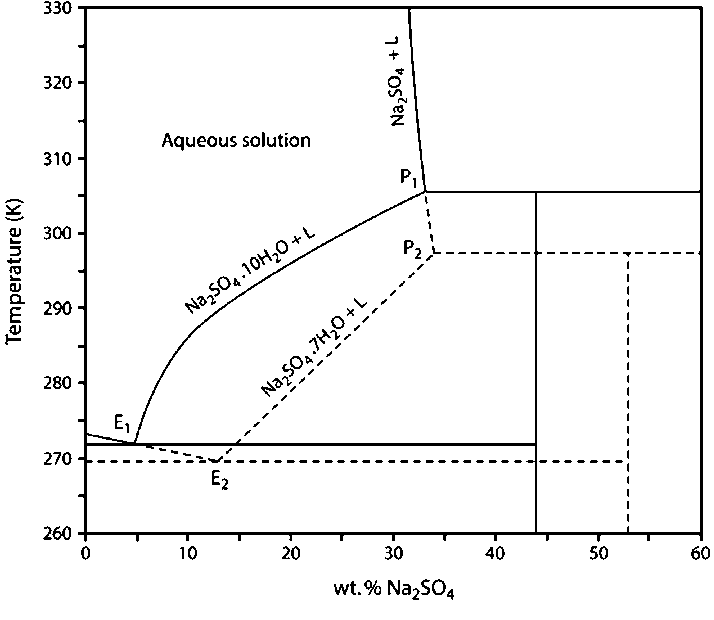
\includegraphics[scale=1.00]{h2o-diagram.png}
\caption{Диаграмма системы соль-вода на примере сульфата натрия}
\label{}
\end{figure}


Излом на графике обусловлен тем, что растворимость $Na_2SO_4\cdot10H_2O$ является эндотермическим процессом. В то же время при 32 градусах он инконгруэнтно (с разложением) плавится. Выше этой температуры величина растворимости обусловлена равновесием раствора с безводным сульфатом натрия. Переход последнего в гидрат сопряжен со значительным выделением тепла.  Поэтому для $Na_2SO_4\cdot10H_2O$ энтальпия положительна. До тех пор, пока растворимость определяется равновесием декагидрата с раствором, она растет, а после точки перетектики – падает с ростом температуры.

\subsection*{Зависимость растворимости от температуры}

У одних солей растворимость очень сильно растет с ростом температуры, у других менее резко.

У кристаллических веществ может наблюдаться не только увеличение, но и понижение растворимости при нагревании. Это связано со знаком изменения энтальпии в процессе
растворения. 

Разрушение кристаллической структуры вещества при переходе в раствор требует затраты энергии ( эндотермический процесс). Но частицы растворенного вещества химически взаимодействуют с растворителями. Химическое взаимодействие в растворе сопровождается уменьшением энатльпии(экзотермический процесс). 

Суммарное изменение энтальпии процесса растворения может оказаться как положительным, так и отрицательным.

При протекании эндотермического процесса происходит увеличение растворимости с ростом температуры.

\subsection*{Факторы, влияющие на растворимость}
\begin{itemize}
\item Растворимость веществ во многом обуславливается силой и характером их взаимодействия с молекулами растворителя.

\item Растворимость веществ значительно повышается, если они способны образовывать с растворителем водородные и донорно-акцепторные связи.

\item Диэлектрическая проницаемость растворителя является одним из наиболее важных факторов, влияющих на растворимость.

\item Природа смешиваемых веществ (полярные с полярными, неполярные с неполярными)
\end{itemize}
\textbf{Криогидратная точка} - точка, соответствующая эвтектике для системы соль-вода.





\section*{Вопрос № 15.}
\subsection*{Теория кислот и оснований}
\subsubsection*{Теория Аррениуса}
1887г Аррениус: 
кислотами называются вещества, которые в водном растворе диссоциируют с образованием ионов водорода, а основания - вещества, диссоциирующие с образованием ионов гидроксила.

Позже теория была скорректирована. Протон, обладающий чрезвычайно малым радиусом порядка  $10^{-7} $ А, не способен к самостоятельному существованию в растворе. Обладая огромной поляризующей способностью, он в любой момент времени оказывается локализованным на каком-либо электроотрицательном атоме, имеющем неподеленную электронную пару. Таким образом, в водных растворах кислот образуются ионы гидроксония ( $H_3O^+ $),  в которых все три протона оказываются эквивалентными.

Минусы: не позволяет описать диссоциацию в апротонных растворителях
\subsubsection*{Теория Бренстеда}


Бренстед предположил считать кислотами вещества, отдающие протон, а основаниями - принимаюзщие его.

В соответствии с этим определением в качестве основания можно рассматривать аммиак, присоединяющий протон по реакции:
 $$NH_3 + H^+ \rightleftarrows NH_4^+ $$

Соответственно ион аммония, напротив, является кислотой. В свете этой теории каждой кислоте соответствует некоторое сопряженное основание:
 $$ A \rightleftarrows H^+ + B$$
 
 Минусы: не объясняет, почему водный раствор $BF_3$ является кислым
 
 \subsubsection*{Теория Льюиса}

 
 Льюис предложил в качестве кислот рассматривать все вещества, которые при образовании ковалентной связи принимают пару электронов. В таком случае основаниями будут являться вещества, отдающие пару электроном при образовании такой же связи.
 
 К кислотам Льюиса относятся координационно ненасыщенные молекулы или ионы, способные достраивать свою координационную сферу за счет присоединения лигандов, соединения, обладающие незавершенной восьмиэлектронной оболочкой, оксиды и галогениды с ненасыщенной координационной оболочкой ($PF_5$, $SbF_5$...) и катионы, способные образовывать комплексные соединения.
 
 К основаниям относятся анионы, включая $OH^-$, и молекулы, способные выступать в комплексных  соединениях в качестве лигандов.
 
 Минусы: невозможно предсказать силу, не может описать классические кислоты.

\subsubsection*{Теория Пирсона}

Пирсон постулировал, что связь между кислотой и основанием не обязательно должна являться ковалентной, а может включать и другие виды взаимодействия (в том числе и ионную связь).

В соответствии с этой теорией к реакциям нейтрализации относится даже процесс образования кристаллической решетки ионами натрия и хлора.

Наиболее ценным в теории Пирсона является представление о наличии жестких и мягких кислот и оснований. 

К жестким относятся частицы с реакционноспособными центрами, обладающие мало деформируемой электронной структурой. Это могут быть катионы с большим зарядом и малым радиусом, а также анионы элементов с высокой электроотрицательностью (F,O,N)(или включающие эти элементы $NH_3$, $ClO_4^-, OH^-$).

Мягкие частицы имеют электронную структуру с высокой поляризуемостью (катионы с d-электронной подкладкой. объемные анионы, лиганды с функциональными группами, включающими атомы с низкой электроотрицательностью и т.д.)

Жесткие основания образуют наиболее прочные связи с жесткими кислотами, и наоборот. Так, например, такие жесткие кислоты, как ионы $B^{3+}$, $Al^{3+}$, $Ti^{4+}$, предпочтительно образуют соли с жесткими основаниями ($O^{2-}$, $F^-$). С другой стороны, такие мягкие кислоты, как $Ag^+$, $Tl^+$, напротив, более склонны к образованию солей с мягкими основаниями, например, с иодид- или сульфид-ионами.

Минусы: излишняя обширность. В соответствии с этой
теорией к реакциям нейтрализации относится
даже процесс образования кристаллической
решетки ионами натрия и хлора.

\subsection*{Автопротолиз. Ионное произведение воды}


Под протолитическими понимаются реакции переноса протона.

Рассмотрим некоторый растворитель AH (где А- некоторый, не обязательно одноатомный анион), имеющиий на протоне некоторый положительный заряд ($\delta^+$). При этом основное взаимодействие A-H несколько ослабеет и становится возможнным перенос протона между двумя молекулами, участвующими в образовании водородной связи. Протекающие процессы могут быть описаны уравнениями:

$$A-H + A-H \rightleftarrows A-H---A-H \rightleftarrows A---H-A-H \rightleftarrows A^- + H_2A^+$$

Вновь образовавшая избыточная связь A-H оказывается слабее исходной. Поэтому  равновесие реакции существенно смещено влево и константа равновесия мала, однако некоторый выигрыш в энтропии обеспечивает протекание такого рода процессов в любых не апротонных растворителях. Это явление получило название автопротолиза. Характерным примером такового является равновесие, устанавливающееся в водном растворе:

$$H_2O + H_2O \rightleftarrows H_3O^+ + OH^-$$

Автопротолизом обусловлена маленькая, но существующая, электропроводимость чистой воды. Поскольку концентрация воды величина постоянная, константа равновесия может быть выражена соотношением: 
$$K_{\alpha} = \left[H_3O^+\right]\left[OH^-\right]$$

Константа автопротолиза является ионным произведением воды.

Константа автопротолиза увеличивается  с ростом температуры. Это соотношение оказывается справедливым также для любых растворов кислот, солей и оснований, поскольку концентрация воды во вспх этих системах меняется сравнительно слабо и близка к 55,5 моль/л. При растворении таких веществ в воде меняется ионная сила раствора, что приводит к величинам коэффициентов активности для катионов, отличных от единицы.

\subsection*{Сильные и слабые кислоты. Факторы, определяющие силу кислот}

Направление смещения кислотно-основного равновесия определятся следующим правилом:

Кислотно-основные равновесия смещены в сторону более слабой кислоты и более слабого основания.

Кислота тем сильнее, чем легче она отдает протон, а основание тем сильнее, чем легче оно принимает протон и прочнее его удерживает. Молекула (или ион) слабой кислоты не склонна отдавать протон, а молекула (или ион) слабого основания не склонна его принимать, этим и объясняется смещение равновесия в их сторону. Силу кислот, а также силу оснований можно сравнивать только в одном и том же растворителе
Так как кислоты могут реагировать с разными основаниями, то соответствующие равновесия будут смещены в ту или иную сторону в разной степени. Поэтому для сравнения силы разных кислот определяют, насколько легко эти кислоты отдают протоны молекулам растворителя. Аналогично определяется и сила оснований.

Сила кислоты – характеристика кислоты, показывающая, насколько легко кислота отдает протоны молекулам данного растворителя.
Сила основания – характеристика основания, показывающая, насколько прочно основание связывает протоны, оторванные от молекул данного растворителя.

 И кислоты, и основания можно сравнивать между собой по силе в водных растворах. В одном и том же растворителе сила кислоты в значительной степени зависит от энергии рвущейся связи А-Н, а сила основания – от энергии образующейся связи В-Н.

Для количественной характеристики силы кислоты в водных растворах можно использовать константу кислотно-основного равновесия обратимой реакции данной кислоты с водой: 
$$K = \frac{\left[A^-\right]\left[H_3O^+\right]}{\left[HA\right]\left[H_2O\right]}$$

Для характеристики силы кислоты в разбавленных растворах, в которых концентрация воды практически постоянна, пользуются константой кислотности: 
$$K_k = \frac{\left[A^-\right]\left[H_3O^+\right]}{\left[HA\right]}$$

Совершенно аналогично для количественной характеристики силы основания можно использовать константу кислотно-основного равновесия обратимой реакции данного основания с водой:
$$K = \frac{\left[HA\right]\left[OH^-\right]}{\left[A^-\right]\left[H_2O\right]}$$

а в разбавленных растворах – константу основности: 
$$K_o = \frac{\left[HA\right]\left[OH^-\right]}{\left[A^-\right]}$$
Основание тем сильнее, чем слабее сопряженная кислота. И наоборот, кислота тем сильнее, чем слабее сопряженное основание.

Чем же определяется сила кислоты? Возьмем случай, когда молекула электронейтральна.

В первую очередь, соотношением донорных свойств неподеленной электронной пары и склонности к диссоциации связи Э-H.

Активность первой падает, а второй - возрастает при продвижении по периоду таблицы Менделеева слева-направо. Это определяется ростом электроотрицательности связанного с протоном атома, а во-вторых тем, что донорная способность электронных пар тем выше, чем меньше их число. В этом же ряду понижается электронная плотность связи Э-H, что облегчает ее диссоциацию.

При продвижению сверху вниз по подгруппе донорные свойства электронной пары убывают в связи с уменьшением "склонности к $sp^3$ - гибридизации". Это явление можно объяснить тем, что ввиду увеличения размера орбиталей и понижения разницы между энергией последней заполненной (p) и последующей вакантной (чаще всего d) орбитали электронная плотность этой пары оказывается существенно более делокализованной. С другой стороны, с ростом радиуса элемента прочность связи Э-H существенно убывает.

\subsection*{Концентрация ионов водорода. pH.}

Водные растворы могут быть нейтральными, кислыми или щелочными. В кислых растворах содержится избыток ионов $H^+$, а в щелочных – избыток ионов $OH^-$. В нейтральных растворах количество этих ионов всегда одинаково и при этом чрезвычайно мало – по $10^{-7}$ моль/л каждого иона. Низкая концентрация ионов $H^+$ и $OH^-$ в нейтральном растворе вполне объяснима – ведь эти ионы охотно реагируют друг с другом, поскольку в результате образуется прочное, малодиссоциированное соединение $H_2O$. Таким образом, в нейтральном растворе присутствуют только те ионы $H^+$ и $OH^-$, которые образовались из самой воды естественным путем, в результате ее обратимой диссоциации.

Для воды и ее растворов при неизменной температуре произведение концентраций ионов водорода и гидроксид-ионов есть величина постоянная. Эта постоянная величина называется ионным произведением воды $K_w$

$$K_w = \left[H^+\right]\left[OH^-\right] = 10^{-14}$$

Водородный показатель показывает, что кислотность или щелочность растворов можно выразить через концентрацию одних только ионов водорода $H^+$.

Водородный показатель определяется следующим образом: рН раствора равен обратному логарифму от концентрации ионов водорода в этом растворе.

$$pH = -\lg\left[H^+\right]$$

\subsection*{Гидратированные ионы, как пример слабых кислот.}


По определению Льюиса, катион любого элемента склонен к образованию координационной связи с электронными парами лигандов и, следовательно, является кислотой.

Действительно, в водных растворах катионы координируют вокруг себя молекулы воды.При этом за счет образования координационных связей, электронная плотность с последних смещается к металлу. Это приводит к увеличению положительного заряда на протонах воды и повышает веротность кислотной диссоциации по следующей схеме:

$$\left[(H_2O)_n MOH_2\right]^{z+} + OH_2 \rightleftarrows \left[(H_2O)_n MOH-H---OH_2\right]^{z+} \rightleftarrows \left[(H_2O)_n MOH\right]^{z-1} + H_3O^+$$

\section*{Вопрос 18}
\subsection*{Кристаллизация из расплава (ТХ-диаграммы)}
Диаграмма плавкости веществ с неограниченной растворимостью в жидком и полной нерастворимостью в твердом состоянии.

Этот тип диаграмм характерен для веществ, заметно отличающихся структурой кристаллов.

Диаграмма температура–состав строится на основании кривых охлаждения (нагревания). Кривые охлаждения – графическое изображение зависимости температуры от времени для исходных чистых веществ A и B и их смесей различного состава. Вид этих кривых свидетельствует о наличии или отсутствии фазовых превращений при некоторых определенных температурах или в интервале температур 
\begin{figure}[htp]
\centering
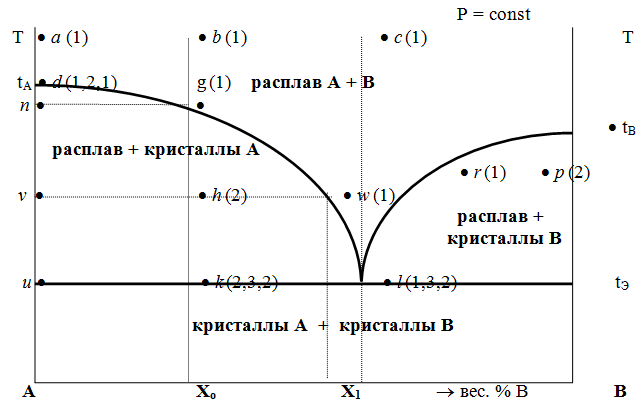
\includegraphics[scale=.500]{cristallization-diagram.png}
\caption{}
\label{}
\end{figure}

Весьма часто твердая фаза, выделяющаяся при охлаждении расплавов, состоит из кристаллов, образуемых обоими компонентами. Такая однородная система имеет переменный состав и называется твердым раствором. Твердые растворы – системы однофазные, подобно обычным жидким растворам, но в отличие от последних имеют кристаллическую структуру.

\begin{figure}[htp]
\centering
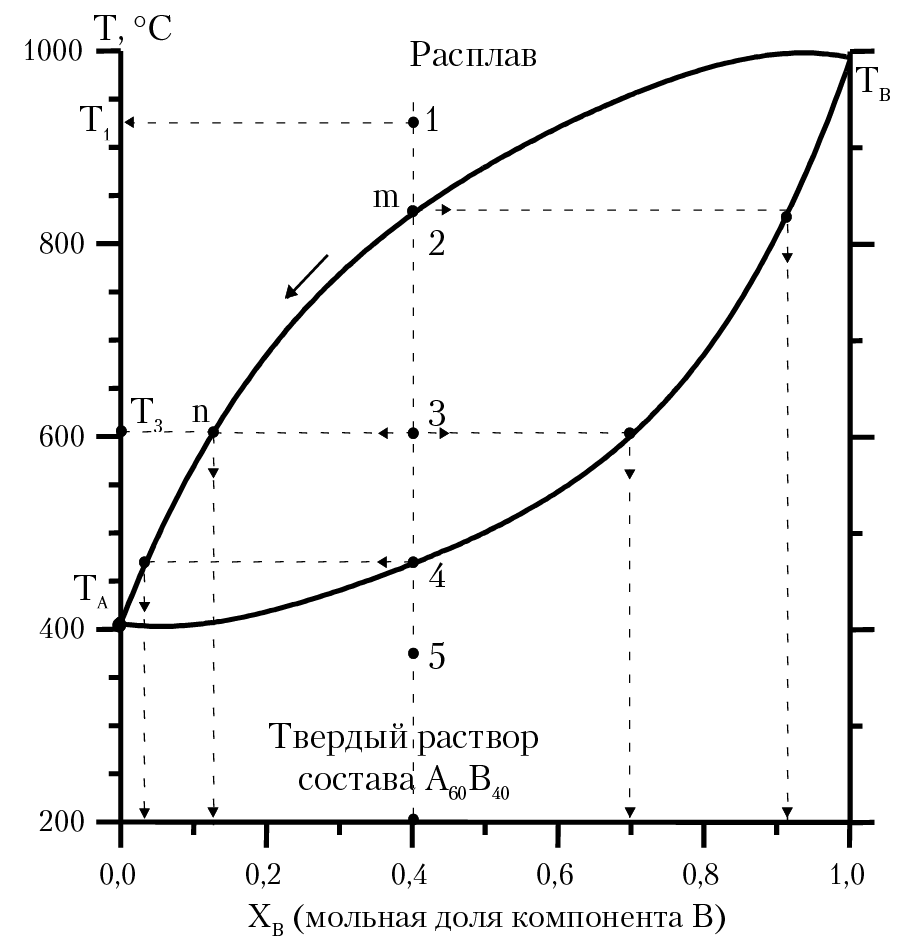
\includegraphics[scale=.500]{cristallization-diagram2.png}
\caption{}
\label{}
\end{figure}

Неограниченной взаимной растворимостью в твердом состоянии обладают вещества, имеющие близкие значения атомных или ионных радиусов, энергии химической связи, сходное строение электронных оболочек и одинаковый тип кристаллической решетки (изоморфные вещества). Примерами таких систем могут служить $Au-Ag$, $Cu-Au$, $Se-Ge$, $NaCl-NaBr$ и другие.

\subsection*{Зонная плавка}

Зонная плавка (зонная перекристаллизация) - метод очистки твёрдых веществ, основанный на различной растворимости примесей в твёрдой и жидкой фазах. Метод является разновидностью направленной кристаллизации, от которой отличается тем, что в каждый момент времени расплавленной является некоторая небольшая часть образца. Такая расплавленная зона передвигается по образцу, что приводит к перераспределению примесей. Если примесь лучше растворяется в жидкой фазе, то она постепенно накапливается в расплавленной зоне, двигаясь вместе с ней. В результате примесь скапливается в одной части исходного образца. По сравнению с направленной кристаллизацией этот метод обладает большей эффективностью. Метод был предложен Уильямом Гарднером Пфанном в 1952 году и с тех пор завоевал большую популярность. В настоящее время метод используется для очистки более 1500 веществ.

Распределение примеси характеризуется коэффициентом распределения, который равен

$$ K={\frac {C_{S}}{C_{L}}}$$

где $C_S$ - концентрация примеси в твёрдой фазе, $C_L$ - концентрация примеси в жидкой фазе.

Иногда вместо коэффициента распределения $K$ используют коэффициент разделения $\alpha$, который равен

$$\alpha ={\frac {C_{S}(1-C_{L})}{C_{L}(1-C_{S})}}$$

Примеси, для которых коэффициент распределения K < 1, концентрируются в расплавленной зоне и вместе с ней перемещаются к концу слитка. С другой стороны от расплавленной зоны образуются слои вещества, более чистого относительно примесей, для которых K < 1. Те примеси, для которых K > 1, наоборот, концентрируются в начале слитка. Если осуществить многократное прохождение расплавленной зоны, то примеси с K < 1 соберутся в конце слитка. Для примесей с К > 1 метод мало эффективен. Самые чистые части слитка (из середины) используются для изготовления приборов. Таким методом можно очистить германий до образцов с удельным сопротивлением порядка 70 Ом·см, в которых остаётся примерно один атом примеси на 1010 атомов германия.

Если расплав вступает в реакцию с материалом тигля (лодочки), или очищаемое вещество имеет высокую температуру плавления ($>1500^o C$), применяют бестигельную зонную плавку.

Метод обладает рядом недостатков. Основной недостаток - невозможность масштабирования, так как скорость процесса определяется скоростью диффузии примеси. Поэтому метод применяется для конечной стадии очистки при получении особо чистых веществ. Максимальные габариты лодочки - длина 50 см, толщина - 2-3 см, длина расплавленной зоны - 5 см.
\subsection*{ТХ-диаграмма системы жидкость-пар, дистилляция}
TX-диаграмма системы жидкость-пар изображена ниже:
\begin{figure}[htp]
\centering
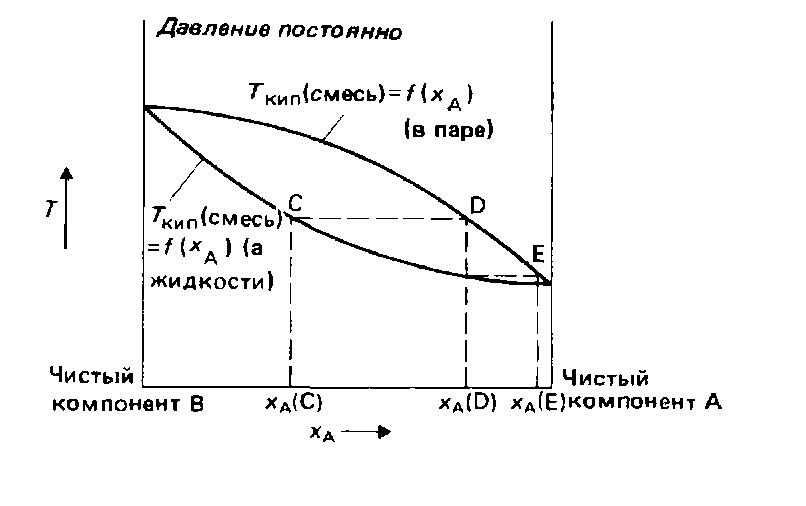
\includegraphics[scale=1.50]{vapor-diagram.png}
\caption{}
\label{}
\end{figure}

Две линии на ней - начало(снизу) и конец(сверху) кипения. Внизу - жидкость, посередине - равновесие жидкости и пара, сверху - пар. 

\textbf{Дистилляция} - перегонка, испарение жидкости с последующим охлаждением и конденсацией паров. Дистилляцию рассматривают прежде всего как технологический процесс разделения и рафинирования многокомпонентных веществ - в ряду других процессов с фазовым превращением и массообменом: сублимация, кристаллизация, жидкостная экстракция и некоторых других. 

Различают дистилляцию с конденсацией пара в жидкость (при которой получаемый дистиллят имеет усреднённый состав вследствие перемешивания) и дистилляцию с конденсацией пара в твёрдую фазу (при которой в конденсате возникает распределение концентрации компонентов). 

Продуктом дистилляции является дистиллят или остаток (или и то, и другое) - в зависимости от дистиллируемого вещества и целей процесса. Основными деталями дистилляционного устройства являются обогреваемый контейнер (куб) для дистиллируемой жидкости, охлаждаемый конденсатор (холодильник) и соединяющий их обогреваемый паропровод.

Существуют разные вариации на тему, вроде перегонки с водяным паром, но это экзотика, которая врядли кому-то нужна.


\subsection*{Возгонка, РТ-диаграммы перегоняемых веществ}

Обратным процессом является десублимация. Примером десублимации являются такие атмосферные явления, как иней на поверхности земли и изморозь на ветвях деревьев и проводах.

На диаграмме состояний (де)сублимация - это переход линии, соединяющей абсолютный ноль и тройную точку.

\begin{figure}[htp]
\centering
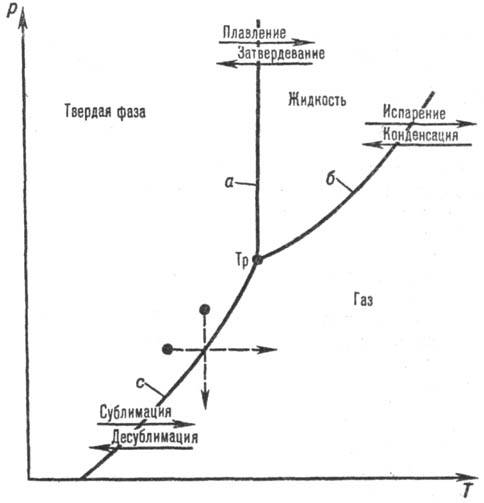
\includegraphics[scale=.50]{sublimation.jpg}
\caption{}
\label{}
\end{figure}

Сублимацию применяют в химии для очистки некоторых веществ, например иода и бензойной кислоты.

Схема установки для сублимации изображена ниже.
\begin{figure}[htp]
\centering
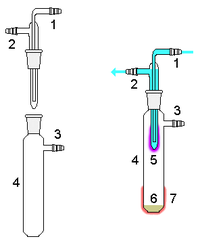
\includegraphics[scale=1.50]{sublimation2.png}
\caption{}
\label{}
\end{figure}

\begin{enumerate}
\item вход воды для охлаждения
\item выход воды для охлаждения
\item выход для вакуума
\item сублимационная камера
\item продукт
\item очищаемое вещество
\end{enumerate}


\subsection*{Транспортные реакции}
Этот метод широко используется при получении особо чистых веществ для полупроводниковой техники и радиоэлектроники. Принцип его состоит в том, что очищаемое твердое или жидкое вещество $А$, взаимодействуя по обратимой реакции с газообразным веществом $В$, образует газообразный продукт $С$, переносимый (транспортируемый) в другую часть системы, где вследствие изменения условий происходит его разложение с выделением чистого вещества $А$:
$$A + B \rightleftarrows C$$

Классическим примером транспортной реакции является очистка металлического никеля через его карбонил (метод Монда). Порошок никеля обрабатывают при $45-50 ^oС$ окcидом углерода:
$$Ni + 4CO \rightleftarrows \left[Ni(CO)_4\right]$$

Газообразный $[Ni(CO)_4]$ поступает в другую часть реакционного аппарата, где при $180-200 ^oС$ разлагается, давая чистый никель, а $СО$ снова направляют в процесс.

Метод транспортных реакций применяется для получения различных чистых веществ как простых, так и сложных. В качестве транспортирующего агента часто используют галогены, галогеноводороды, водяной пар, кислород, водород и др. Например, при получении особо чистых $Ni$, $Cu$, $Fе$, $Cr$, $Si$, $Ti$, $Hf$, $Th$, $V$, $Nb$, $Та$ и $U$ применяют иод.

Направление транспорта (из зоны с низкой температурой в зону с высокой температурой или наоборот) определяется термодинамическими свойствами (знаком теплового эффекта).

При экзотермических реакциях транспорт вещества производится в более нагретую зону, как в приведенном примере с очисткой Ni. Метод транспортных реакций удобен для очистки от элементов, отличающихся по своим химическим свойствам от основного элемента.

Для глубокой очистки от элементов-аналогов он мало пригоден. Достоинством транспортных реакций является возможность проведения всех операций в стерильных условиях, поскольку эти реакции проходят в замкнутом объеме и без больших количеств реагентов.

\subsection*{Хроматография и адсорбция. Экстракция. Ионный обмен} 
\textbf{Хроматография} -  метод разделения и анализа смесей веществ, а также изучения физико-химических свойств веществ. Основан на распределении веществ между двумя фазами - неподвижной (твёрдая фаза или жидкость, связанная на инертном носителе) и подвижной (газовая или жидкая фаза, элюент). Название метода связано с первыми экспериментами по хроматографии, в ходе которых разработчик метода Михаил Цвет разделял ярко окрашенные растительные пигменты. Опыт цвета показан ниже - он делил хлорофиллы, ксантины и что-то еще в этом духе.

\begin{figure}[htp]
\centering
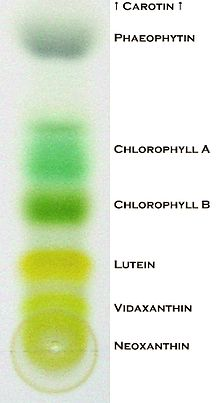
\includegraphics[scale=.5]{chromatorgamm.jpg}
\caption{}
\label{}
\end{figure}

Существует дикое количество видов, по агрегатному состоянию фаз, движущей силе(электрохроматография, ВЭЖХ и т.д.), механизму сорбции(хемосорбция, молекулярные сита, и т.д.), форме оборудования(тонкослойная, колоночная, капиллярная), но не думаю, что их от нас хотят все услышать, тем более, что идея везде одна.

\textbf{Адсорбция} -  самопроизвольный процесс увеличения концентрации растворённого вещества у поверхности раздела двух фаз (твёрдая фаза - жидкость, конденсированная фаза - газ) вследствие нескомпенсированности сил межмолекулярного взаимодействия на разделе фаз. Адсорбция является частным случаем сорбции, процесс, обратный адсорбции - десорбция.

Поглощаемое вещество, ещё находящееся в объёме фазы, называют адсорбтив, поглощённое - адсорбат. В более узком смысле под адсорбцией часто понимают поглощение примеси из газа или жидкости твёрдым веществом (в случае газа и жидкости) или жидкостью (в случае газа) - адсорбентом. При этом, как и в общем случае адсорбции, происходит концентрирование примеси на границе раздела адсорбент-жидкость либо адсорбент-газ. Процесс, обратный адсорбции, то есть перенос вещества с поверхности раздела фаз в объём фазы, называется десорбция. Если скорости адсорбции и десорбции равны, то говорят об установлении адсорбционного равновесия. В состоянии равновесия количество адсорбированных молекул остается постоянным сколько угодно долго, если неизменны внешние условия (давление, температура и состав системы).

\textbf{Экстракция} - это извлечение вещества из раствора или сухой смеси с помощью растворителя (экстрагента), практически не смешивающегося с исходной смесью.

Экстракция может быть разовой (однократной или многократной) или непрерывной (перколяция).

Простейший способ экстракции из раствора - однократная или многократная промывка экстрагентом в делительной воронке. Делительная воронка представляет собой сосуд с пробкой и краном для слива нижнего слоя жидкости. Для непрерывной экстракции используются специальные аппараты - экстракторы, или перколяторы.

Для извлечения индивидуального вещества или определённой смеси (экстракта) из сухих продуктов в лабораториях широко применяется непрерывная экстракция по Сокслету.

В лабораторной практике химического синтеза экстракция может применяться для выделения чистого вещества из реакционной смеси или для непрерывного удаления одного из продуктов реакции из реакционной смеси в ходе синтеза.

Экстракция применяется в химической, нефтеперерабатывающей, пищевой, металлургической, фармацевтической и других отраслях, в аналитической химии и химическом синтезе.

\textbf{Ионный обмен} - это обратимая химическая реакция, при которой происходит обмен ионами между твердым веществом (ионитом) и раствором электролита. Ионный обмен может происходить как в гомогенной среде (истинный раствор нескольких электролитов), так и в гетерогенной, в которой один из электролитов является твёрдым (при контакте раствора электролита с осадком, ионитом и др.).

\emph{Катионный обмен} - частный случай ионного обмена, под которым в химии понимают обратимый процесс стехиометрического обмена ионами между двумя контактирующими фазами.

Ионный обмен используется в химии для замены одного иона на другой, с тем же знаком заряда.
\subsection*{Коэффициент распределения}

Коэффициент разделения (коэффициент распределения) - концентрационная характеристика фазового превращения или фазового равновесия двух- или многокомпонентного вещества. Термин введен около 1950 г. для рассмотрения процессов с фазовым превращением и массообменом (дистилляция, сублимация, кристаллизация, жидкостная экстракция и некоторые другие) как технологических процессов разделения и рафинирования двух- и многокомпонентных веществ. В первую очередь рассматриваются так называемые равновесный, кинетический и эффективный коэффициенты разделения (распределения).

$$K = \frac{C_A^1}{C_A^2}$$
$C_A^1$ - равновесная концентрация вещества в первой фазе\\
$C_A^2$ - равновесная концентрация вещества во второй фазе\\
$K$ - коэффициент распределения

Написанное выше верно для идеального случая - когда фазы в равновесии, то есть прошло бесконечное время. В реальности исползуется коэффициент, в котором не равновесные, а реальные - экспериментальные или литературные концентрации.


\section*{Вопрос 22}

\subsection*{Электролиз растворов и расплавов}

Если потенциал пары $M^{n+}/M$ выше 0.413 B, электролиз будет приводить к выделению на катоде водорода. Поэтому щелочные, щелочноземельные и многие другие металлы нельзя выделить электролизом растворов.

Кислород выделяется на аноде при электролизе растворов фторидов, у которых потенциал окисления существенно больше, чем у кислорода. Выделение на аноде кислорода происходит и при электролизе солей кислородсодержащих кислот.

Функция электролита: перенос тока через раствор, существенно ускоряя процесс электролиза.

Чистота продуктов электролиза существенно зависит от подаваемого напряжения, поскольку с его увеличением возникает возможность выделения примесей. При электролизе расплавов снимается ограничение в предельных потенциалах выделения металла на катоде и электроотрицательных элементов на аноде. Все расплавы являются сильными электролитами. 

\subsection*{Источники тока}
\subsubsection*{гальванические элементы}
Простейший источник тока - гальванический элемент. Его недостатками являются присутствие жидкости, малое выходное напряжение и малая ёмкость. Цинковые батарейки характеризуются низким выходным напряжением и являются необратимыми - их нельзя перезарядить. 
\subsubsection*{Свинцовый аккумулятор}
Принцип работы свинцово-кислотных аккумуляторов основан на электрохимических реакциях свинца и диоксида свинца в водном растворе серной кислоты.

При подключении к электродам аккумулятора внешней нагрузки начинается электрохимическая реакция взаимодействия оксида свинца и серной кислоты, при этом металлический свинец окисляется до сульфата свинца (в классическом варианте аккумулятора). Проведённые в СССР исследования показали, что при разряде аккумулятора протекает как минимум 60 различных реакций, порядка 20 из которых протекают без участия кислоты электролита.

Электрохимические реакции (слева направо - при разряде, справа налево - при заряде):

Реакции на катоде:
$$PbO_{2}+SO_{4}^{2-}+4H^{+}+2e^{-}\leftrightarrows PbSO_{4}+2H_{2}O$$
Реакции на аноде:
$$Pb+SO_{4}^{2-}-2e^{-}\leftrightarrows PbSO_{4}$$

Преимущества свинцового аккумулятора:
\begin{itemize}
 \item Приличный ресурс
 \item \emph{Огромная} допустимая сила тока
 \item Напряжение около 2 В - больше, чем для цинкового элемента
 \item Аккумулятор можно перезарядить
 \end{itemize}
 
 Недостатки:
 \begin{itemize}
 \item Используется агрессивный электролит (H2SO4)
 \item Используется свинец, тяжелый металл, так, на минуточку
\end{itemize}

\subsubsection*{Источник тока на основе твёрдого электролита (например, AgI)} 

Преимущества:
 \begin{itemize}
 \item отсутствие жидкой фазы, высокий коэффициент полезного действия и возможность перезарядки\end{itemize}
 
 Недостатки:
 \begin{itemize}
 \item низкое напряжение – менее 1В. 
 \item Для повышения рабочего напряжения до 3В серебро заменяют на более активный литий, а йод на кислород, содержащийся в соединениях переходных элементов
 \end{itemize}
 \subsubsection*{Топливные элементы}

В топливных элементах водород и кислород разделяются прослойкой материала с проводимостью по ионам водорода и нанесёнными с двух сторон слоями катализатора. Преимуществом топливных элементов является компактность, высокий КПД, возможность автономной работы вдали от линий электропередач, или при их выходе из строя. 

Главное преимущество – абсолютная экологическая чистота. Недостатки: низкая устойчивость или низкая электропроводность при комнатной температуре и низкой влажности таких твёрдых электролитов, а также высокая стоимость платинового катализатора и возможностью его отравления даже следами СО, который практически всегда присутствует в среде.

\section*{Вопрос №24}

\subsection*{Скорость химической реакции}

Многое удается узнать о химических реакциях, изучая скорость их протекания и факторы, от которых она зависит. Этим занимается раздел химии, называемый химической кинетикой.

\textbf{Скоростью химической реакции} называется количество вещества, вступающего в реакцию или образующегося при реакции за единицу времени в единице объема системы.

$$V = \frac {dC}{dt}$$

Количество вещества выражают в \emph{молях}, время как правило в \emph{секундах} а объем в \emph{литрах}.

Таким образом, скоростью реакции называют изменение концентрации какого-нибудь вещества, участвующего в реакции, за единицу времени (например, за секунду или за минуту). Отсюда другое определение скорости реакции:

Следовательно, размерность у скорости реакции такая: "моль/л · сек".

За скоростью реакции $$A + B \Rightarrow C$$ можно следить по расходованию одного из реагентов ($A$ или $B$), либо по накоплению продукта ($C$). Здесь мы сталкиваемся с серьезной проблемой: скорость реакции может постоянно изменяться. Действительно, в начале реакции, когда молекул $A$ и $B$ еще много, столкновения между ними происходят гораздо чаще, чем в конце реакции, когда молекул $A$ и $B$ уже намного меньше. Как мы знаем, столкновения молекул являются поводом для реакции между ними. 

\subsection*{Закон действующих масс и константа скорости} 

$$aA + bB \Rightarrow cC$$

$$V = k \left[A\right]^a\left[B\right]^b$$


Скорость реакции прямо пропорциональна произведению концентраций всех реагентов в степенях, равных \emph{порядку реакции} поэтому реагенту. В случае элементарной реакции, порядок равен коэффициенту перед веществом. Коэффициент пропорциональности - константа скорости. Ее размерность зависит от порядка реакции. Выведем кинетические уранения для нулевого, первого и энного порядка. $C^*$ - константа интагрирования, $C_0$ - начальная концентрация вещества. 

\subsection*{Нулевой порядок}
$$\frac{dC}{dt} = -kC^0 = -k$$
$$\int dC = -\int kdt$$
$$C = -kt + C^*$$
$$C = C_0 - kt$$

\subsection*{Первый порядок}
$$\frac{dC}{dt} = -kC^1 = -kC$$
$$\int \frac{dC}C = -\int kdt$$
$$ln C = -kt + C^*$$
$$C = e^{-kt}\cdot e^{C^*}$$
$$C = C_0e^{-kt}$$

\subsection*{Энный порядок}
$$\frac{dC}{dt} = -kC^n = -kC$$
$$\int \frac{dC}C^n = -\int kdt$$
$$-\frac{1}{(n-1)C^{n-1}} = -kt + C^*$$
$$-\frac{1}{(n-1)C^{n-1}} = -kt - \frac{1}{(n-1)C_0^{n-1}}$$
$$ \frac 1{C^{n-1}} = +kt(n-1) + \frac1{C_0^{n-1}}$$

\subsection*{Связь кинетики и константы равновесия}

Что такое равновесие? Это, с точки зрения кинетики, равенство скоростей прямой и обратной реакций. Запишем это:
$$aA + bB \Rightarrow cC + dD$$
$$K =\frac{\left[C\right]^c\left[D\right]^d}{\left[A\right]^a\left[B\right]^b}$$
$$V_1 = k1 \left[A\right]^a\left[B\right]^b$$
$$V_{-1} = k_{-1}\left[C\right]^c\left[D\right]^d$$
$$\frac{V_1}{V_{-1}} = \frac{k1 \left[A\right]^a\left[B\right]^b}{k_{-1}\left[C\right]^c\left[D\right]^d} = 1$$
$$\frac 1K\frac{k_1}{k_{-1}} = 1$$
$$K = \frac{k_1}{k_{-1}}$$
Итак, константа равновесия есть соотношение констант скорости прямой и обратной реакций

\subsection*{Кинетика обратимых реакций}

$$aA + bB \Rightarrow cC + dD$$

Скорость обратимой реакции равна разности скоростей прямой и обратной реакции.

$$V_1 = k1 \left[A\right]^a\left[B\right]^b$$
$$V_{-1} = k_{-1}\left[C\right]^c\left[D\right]^d$$
$$V_{sum} = V_1 - V_{-1} = k1 \left[A\right]^a\left[B\right]^b - k_{-1}\left[C\right]^c\left[D\right]^d$$

По мере протекания двусторонней реакции скорость прямой реакции уменьшается, скорость обратной реакции – увеличивается; в некоторый момент времени скорости прямой и обратной реакции становятся равными и концентрации реагентов перестают изменяться. Таким образом, в результате протекания в закрытой системе двусторонней реакции система достигает состояния химического равновесия; при этом константа равновесия будет равна отношению констант скоростей прямой и обратной реакции - см. предыдущий пункт.


\end{document}


